%==============================================================================
% Sjabloon poster bachproef
%==============================================================================
% Gebaseerd op document class `a0poster' door Gerlinde Kettl en Matthias Weiser
% Aangepast voor gebruik aan HOGENT door Jens Buysse en Bert Van Vreckem

\documentclass[a0,portrait]{hogent-poster}

% Info over de opleiding
\course{Bachelorproef}
\studyprogramme{toegepaste informatica}
\academicyear{2025-2026}
\institution{Hogeschool Gent, Valentin Vaerwyckweg 1, 9000 Gent}

% Info over de bachelorproef
\title{Omzetten van \emph{UML}-diagrammen (\emph{PlantUML}) naar "\emph{configuration management}"-code (\emph{Ansible})}
\subtitle{Onderzoek \& \emph{Proof of Concept}}
\author{Lucas Ludueña-Segre}
\email{lucas.luduenasegre@student.hogent.be}
\supervisor{Alexander Veldeman}
\cosupervisor{Yoeri Rousseaux (District09)}

\specialisation{IT infrastructure engineer}
\keywords{UML, PlantUML, Infrastructure-as-Code, IaC, Vagrant, configuration management, Ansible, converter}
\projectrepo{https://github.com/lucasluduenasegre/plantuml2ansible}

\begin{document}

\maketitle

\begin{abstract}
      Deze bachelorproef onderzoekt hoe men netwerk- en implementatiediagrammen met minimale menselijke interventie kan omzetten tot overeenkomende ``\emph{configuration management}''-ondersteunde omgevingen.
      Er werd hiervoor een \emph{Proof of Concept} \emph{converter} ontwikkeld die, op basis van \emph{PlantUML}-bronbestanden, een \emph{Vagrant}- en \emph{Ansible}-ondersteunde omgeving produceert.
      Hierop werden een aantal testcases uitgevoerd (op basis van opleidingsonderdelen binnen \emph{Toegepaste Informatica}) die de technische haalbaarheid van de onderzoeksdoelstelling aantonen.
      De meerwaarde van deze tool bevindt zich binnen een educatieve context: docenten kunnen labo's sneller implementeren en studenten kunnen infrastructuurideeën gemakkelijker uitproberen.
\end{abstract}

\begin{multicols}{2}

      \section{Introductie}

      Binnen de opleiding \emph{Toegepaste Informatica} op \emph{HOGENT} wordt er binnen het keuzeprofiel ``\emph{IT infrastructure engineer}'' aangeleerd om infrastructuren te beheren, o.a. aan de hand van netwerk- en implementatiediagrammen, die de topologie, software en onderlinge verbindingen van servers voorstellen.

      \textbf{Probleemstelling}: het proces waarbij netwerk- en implementatiediagrammen geïnterpreteerd en omgezet worden tot ``\emph{IaC}''- en ``\emph{configuration management}''-ondersteunde serveromgevingen is, volgens Nicácio \& Petrillo (2020), foutgevoelig en tijdrovend.

      \textbf{Hoofdonderzoeksvraag}: \emph{Hoe kan men een netwerk- en implementatiediagram met minimale menselijke interventie omzetten tot een overeenkomende, gebruiksklare ``}configuration management\emph{''-ondersteunde omgeving?}

      \section{Methodologie}

      \begin{center}
            \captionsetup{type=figure}
            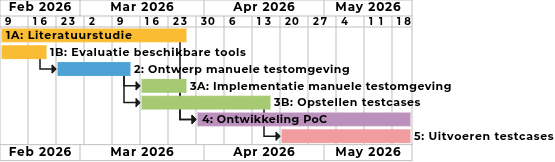
\includegraphics[width=\linewidth]{../graphics/gantt-fases-small.png}
            \captionof{figure}{Fases van de methodologie aan de hand van een GANTT-schema. Fase 1B onderzocht de te gebruiken tools voor de PoC, en de uitvoer voor deze PoC werd gebaseerd op de functionaliteit van de manuele testomgeving (fases 2 en 3A).}
      \end{center}

      \section{\emph{Proof of Concept} (\emph{PlantUML2Ansible})}


      \begin{center}
            \begin{minipage}{\linewidth}
                  \captionsetup{type=figure}
                  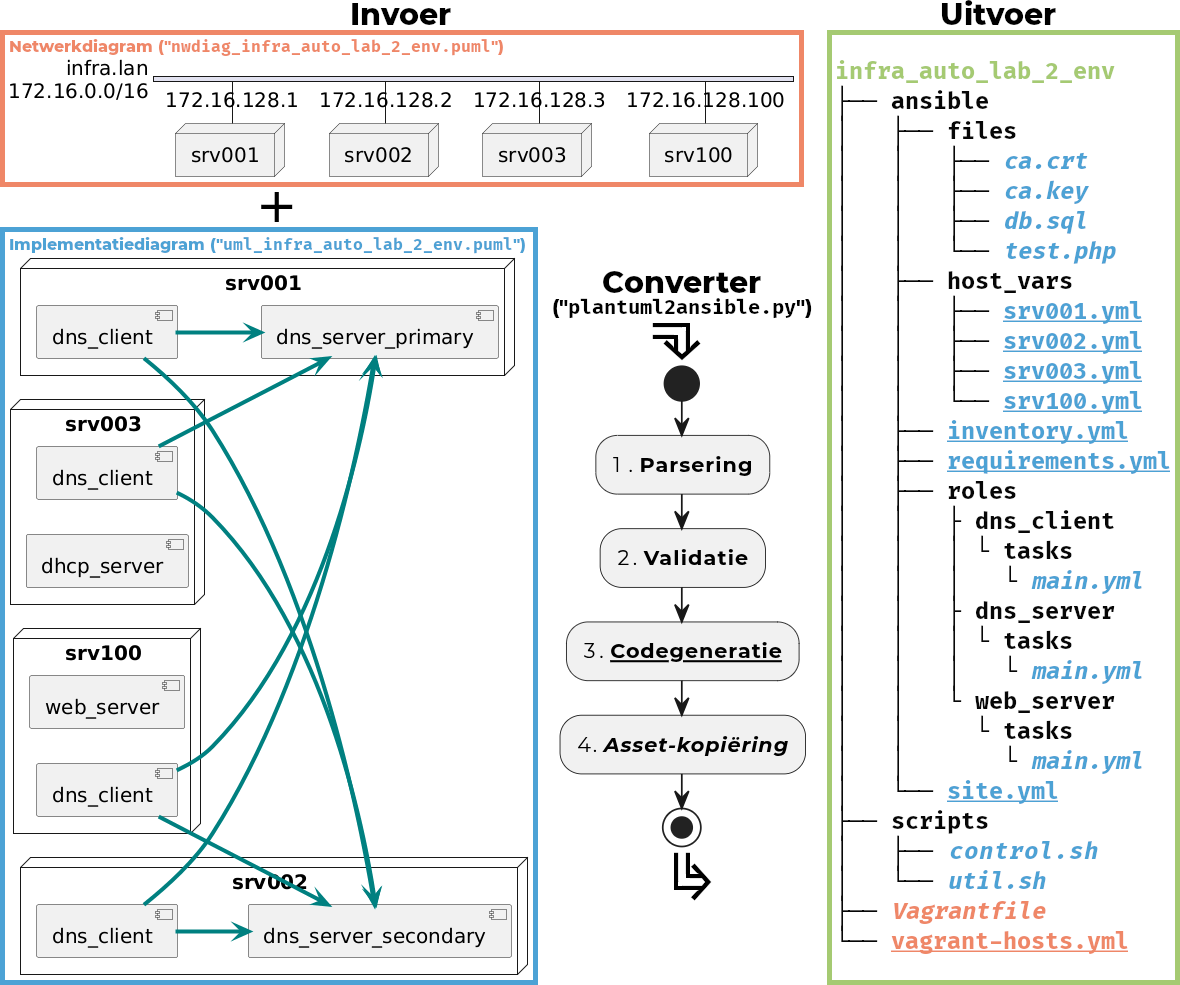
\includegraphics[width=\linewidth]{../graphics/demo.png}
                  \captionof{figure}{Vereenvoudigde werking (invoerbestanden, stappen, uitvoerstructuur) van de \emph{converter} ``\texttt{plantuml2ansible.py}'', met testcase 2 (\emph{Infrastructure Automation}, labo 2) als voorbeeld.}
            \end{minipage}
      \end{center}
      De \emph{converter} ondersteunt twee \emph{gebruiksscenario}'s:

      \begin{description}
            \item[\emph{``full mode''}] (zoals te zien op figuur 2): neemt zowel een netwerk- als implementatiediagram als invoerbestanden. Deze produceert een complete \emph{Vagrant}- én \emph{Ansible}-ondersteunde omgeving (aan de hand van voorgedefinieerde \emph{Ansible}-rollen en een ingebouwde \emph{Ansible} ``\texttt{control}'' node), maar ondersteunt slechts één netwerk.
                  \item[\emph{``IaC-only-mode''}]: neemt enkel een netwerkdiagram als invoer. Deze produceert uitsluitend een \emph{Vagrant}-ondersteunde omgeving én ondersteunt meerdere netwerken (max. 3 IP-adressen per host).
      \end{description}

      \section{Resultaten}

      \begin{description}
            \item[Testcase 1 -- \emph{Cybersecurity Advanced} ("\emph{IaC-only-mode}")]: De volledige labo-omgeving (4 subnetten, 8 beheerde hosts waaronder routers, werkstations en servers) werd succesvol gereproduceerd als \emph{Vagrant}-omgeving (zonder \emph{Ansible}-ondersteuning). Deze kan worden opgestart met het ``\texttt{vagrant up}''-commando.
            \item[Testcase 2 -- \emph{Infrastructure Automation}, labo 2 ("\emph{full mode}")]: Deze omgeving (primaire \& secundaire DNS-server, DHCP-server en webserver) werd volledig gereproduceerd, met uitzondering op de router en workstation. DNS-clients werden ingesteld op basis van verbindingen in het implementatiediagram.
            \item[Testcase 3 -- \emph{Infrastructure Automation}, labo 3 ("\emph{full mode}")]: Dit is een uitbreiding van testcase 2 met een monitoringserver. Monitoringdoelen werden ook geconfigureerd op basis van verbindingen in het implementatiediagram.
      \end{description}
      \section{Conclusie}

      De testresultaten tonen aan dat het \emph{technisch haalbaar} is om op basis van netwerk- en implementatiediagrammen functionele omgevingen te produceren zonder manuele tussenkomst. De kloof tussen de ontwerp- en implementatiefase wordt met deze tool aanzienlijk verkleind.

      De \emph{converter} kent een aantal \textbf{beperkingen}:

      \begin{itemize}
            \item Er wordt maar één netwerk ondersteund binnen ``\emph{full mode}''.
            \item Er is geen routering tussen verschillende netwerken.
            \item Enkel \emph{IPv4}-adressering wordt ondersteund.
            \item Alleen \emph{AlmaLinux 9} kan als gastbesturingssysteem gebruikt worden.
            \item De \emph{converter} houdt slechts rekening met een beperkte subset van de\\\emph{PlantUML}-syntax
      \end{itemize}

      Deze vormen wel een vertrekpunt voor \textbf{toekomstige uitbreidingen}:

      \begin{itemize}
            \item Ondersteuning voor \emph{meerdere netwerken} binnen ``\emph{full mode}'',
                  inclusief configuratie voor routering en bijhorende firewall-regels.
            \item Ondersteuning voor \emph{IPv6}-adressering.
            \item Uitbreiding naar andere \emph{gastbesturingssystemen} (\emph{AlmaLinux 10},
                  \emph{Ubuntu\\Server}, \emph{Alpine Linux}) via meer distributie-agnostische \emph{Ansible}-modules.
            \item Ondersteuning voor andere \emph{IaC-} (\emph{Terraform}, \emph{OpenTofu}) en \emph{configuration management-backends}
                  (\emph{Puppet}, \emph{Chef}).
            \item Formele validatie van invoer en uitvoer via geïntegreerde linters.
      \end{itemize}

\end{multicols}
\end{document}